\documentclass[10pt,a4paper,titlepage]{article}
\usepackage[margin=2.5cm]{geometry}
\usepackage{setspace}	% to use \doublespace
\usepackage{amsmath}
\newcommand\numberthis{\addtocounter{equation}{1}\tag{\theequation}}	% to number a equation using \numberthis in a align* eviroment
\usepackage{cases}
\usepackage{graphicx}
\usepackage{natbib}	% citations
  \bibpunct{(}{)}{;}{a}{,}{,}	% https://en.wikibooks.org/wiki/LaTeX/Bibliography_Management#Citations
\graphicspath{ {../figuras/} }

\usepackage[edtable,displaymath,mathlines]{lineno}		% for line numbering (including tables and equations)
\renewcommand\linenumberfont{\normalfont\bfseries\small}	% change font of line number

\usepackage{caption} 
\captionsetup[table]{singlelinecheck=false}			% to left align table caption
\usepackage{multirow}						% enable row cell spanning 

\renewcommand*{\thefootnote}{\fnsymbol{footnote}}		% change footnote from number to symbol *
%\renewcommand*{\thefootnote}{\arabic{footnote}}		% switch back to arabic number


\title{Mechanistic numerical modeling of solute uptake by plant roots \\ A mechanistic solution for the combined water and solute uptake by plant roots}
\date{January, 2016}
\author{Andre Herman Freire Bezerra
  \thanks{
  Bezerra, A.H.F. and Q. de Jong van Lier, Exact Sciences Dep., ESALQ--Univ. of S\~ao Paulo, 13418-900 Piracicaba, Brazil;
  S.E.A.T.M. van der Zee, Dep. of Environmental Sciences, Wageningen Univ., 6708 PB Wageningen, the Netherlands.
  }
\and Quirijn de Jong van Lier \and Sjoerd E.A.T.M van der Zee}


%% BEGIN DOCUMENT %%%%%%%%%%%%%%%%%%%%%%%%%%%%%%%
\begin{document}
\linenumbers
\maketitle

\section*{Core ideas}
\begin{itemize}
  \item idea 1
  \item idea 2
  \item idea 3
  \item optional idea 4
  \item optional idea 5
\end{itemize}

\section*{Abstract}

% 250 words MAXIMUM!!
A modification in an existing water uptake and solute transport numerical model was implemented in order to allow the model to simulate solute uptake by the roots.
The convection-dispersion equation (CDE) was solved numerically, using a complete implicit scheme, considering a transient state for water and solute fluxes and a soil solute concentration dependent boundary for the uptake at the root surface, based on the Michaelis-Menten (MM) equation.
Additionally, a linear approximation was developed for the MM equation such that the CDE has a linear and a non-linear solution.
A radial geometry was assumed, considering a single root with its surface acting as the uptake boundary and the outer boundary being the half distance between neighboring roots, a function of root density.
The proposed solute transport model includes active and passive solute uptake and predicts solute concentration as a function of time and distance from the root surface.
It also estimates the relative transpiration of the plant, on its turn directly affecting water and solute uptake and related to water and osmotic stress status of the plant.
Performed simulations show that the linear and non-linear solutions result in significantly different solute uptake predictions when the soil solute concentration is below a limiting value ($C_{lim}$).
This reduction in uptake at low concentrations may result in a further reduction in the relative transpiration.
The contributions of active and passive uptake vary with parameters related to the ion species, the plant, the atmosphere and the soil hydraulic properties. 
The model showed a good agreement with an analytical model that uses a linear concentration dependent equation as boundary condition for uptake at the root surface.
The advantage of the numerical model is it allows simulation of transient solute and water uptake and, therefore, can be used in a wider range of situations.
Simulation with different scenarios and comparison with experimental results are needed to verify model performance and possibly suggest improvements.



\section*{Text}

% Must be introduction together with literature review
Crop growth is directly related to plant transpiration, and the closer the cumulative transpiration over a growing season is to its potential value, the higher will be the crop yield. 
Any stress occurring during crop development results in stomata closure and transpiration reduction, affecting productivity. 
Therefore, knowing how plants respond to abiotic stresses like those related to water and salt, and predicting and quantifying them, is important not only to improve the understanding of plant-soil interactions, but also to propose better crop management practices.
The interpretation of experimental data to analyze the combined water and salt stress on transpiration and yield has been shown to be difficult due to the great range of possible interactions between the factors determining the behavior of the soil-plant-atmosphere (SPA) system.
Modeling has been shown to be an elucidative manner to analyze the involved processes and mechanisms, providing insight in the interaction of water and salt stress.

Analytical models describing transport of nutrients in soil towards plant roots usually consider steady state conditions with respect to water flow to deal with the high non-linearity of soil hydraulic functions. 
Several simplifications (assumptions) are needed regarding the uptake of solutes by the roots, most of them also imposed by the non-linearity of the influx rate function. 
Consequently, although analytical models describe the processes involved in transport and uptake of solutes, they are only capable of simulating water and solute flow just for specific boundary conditions.
Therefore, applying these models in situations that do not exactly correspond to their boundary condition may lead to a rough approximation but may also result in erroneous predictions.
Many of the available analytical solutions include special math functions (Bessels, Airys or infinite series, for example) that need, at some point, numerical algorithms to compute results.
For the case of the convection-diffusion equation, even the fully analytical solutions are restricted by numerical procedures, although with computationally efficient and reliable results.

As a substitute to analytical solutions, numerical modeling allows more flexibility when dealing with non-linear equations, being an alternative to better cope with diverse boundary conditions. 
The functions can be solved considering transient conditions for water and solute flow but with some pullbacks regarding numerical stability and more processing to perform calculations.
In general, numerical models use empirical functions that relate osmotic stress to some electric conductivity of the soil solution. 
The parameters of these empirical models depend on soil, plant and atmospheric conditions in a range covered by the experiments used to generate data for model calibration. 
Using these models out of the measured range is not recommended and, in these cases, a new parameter calibration should be done.
Physical/mechanistic models for the solute transport equations describe the involved processes in a wider range of situations since it is less dependent on experimental data, giving more reliable results.

% Thesis objective
%The objective of this thesis is to present a modification of the model of root water uptake and solute transport proposed by \cite{liersolute}.
%This modification allows the model to take into account plant solute uptake.
%To do so, a numerical mechanistic solution for the equation of convection-dispersion will be developed that considers transient flow of water and solute, as well as root competition.
%A soil concentration dependent solute uptake function as boundary condition at the root surface was assumed.
%In this way, the new model allows prediction of active and passive contributions to the solute uptake, which can be used to separate ionic and osmotic stresses by considering solute concentration inside the plant. 
%The proposed model is compared with the original model, with a constant solute uptake numerical model and with an analytical model that uses a steady state condition for water content. 

% Paper objective
In this study, we develop a mechanistic based numerical scheme to solve the convection-dispersion equation for radial root solute extraction.
The model uses the water uptake scheme from \cite{lierwater}.
Assuming a boundary condition at root surface of concentration dependent solute uptake, the solution for the CDE considers transient flow of water and solute, as well as root competition.
The model allows prediction of active and passive contributions to the solute uptake, which can be used to separate ionic and osmotic stresses by considering solute concentration inside the plant.


\def\clim{$C_{lim}$}
\def\c2{$C_2$}
\def\uwc{(m$^3$ m$^{-3}$) }
\def\uhead{(m) }
%\renewcommand{\arraystretch}{2.0}	% increasespace between elements of all arrays

\section*{MATERIAL AND METHODS}

\subsection*{Hydraulic Properties and Soil}

Water uptake was analyzed using hydraulic data for three topsoils from the Dutch Staring series \citep{wosten} as listed in Table \ref{soils}.
The \cite{genuchten80} equation system was used to describe $K$--$\theta$--$h$ relations for these soils:

\begin{equation}
\label{eq_theta}
\theta(h) = \theta_r + {\theta_s-\theta_r \over [1+|\alpha h|^n]^{1-(1/n)}}
\end{equation}

\begin{equation}
\label{eq_K}
K(\theta) = K_{s} \Theta^\lambda [1-(1-\Theta^{n/(n-1)})^{(1-(1/n)})]^2 
\end{equation}
%
where $\theta$ \uwc is the water content, $K$ (m s$^{-1}$) and $K_s$ (m s$^{-1}$) are respectively the hydraulic conductivity and the saturated hydraulic conductivity, $h$ is the pressure head (m), $\Theta$ (--) is the effective saturation defined by ${(\theta - \theta_r) \over (\theta_s-\theta_r)}$; $\theta_s$ \uwc and $\theta_r$ \uwc are the saturated and residual water contents, respectively; and $\alpha$ (m$^{-1}$), $\lambda$ (--) and $n$ (--) are empirical parameters.

% Table with soil types

% macro pmb to bold math symbols
\long\def\pmb#1{\setbox0=\hbox{#1}\copy0\kern-\wd0%
\kern0.02em\raise0.02ex\copy0\kern-\wd0\kern0.02em\box0}

{\tenpoint
\midinsert\medskip \label[soils]
\caption/t {Soil hydraulic parameters used in simulations}
\def\tabiteml{\hbox to 4pt{}}  % left material before each \table item
\def\tabitemr{\hbox to 4pt{}}
\ctable{lcccccccc}{
\crl\hfil 
{\bf Staring}	& {\bf Textural}& {\bf Reference}	& \pmb{$\theta_r$}	& \pmb{$\theta_s$}	& \pmb{$\alpha$}& {\bf l}	& {\bf n}	& \pmb{$K_s$}		\cr 
{\bf soil ID}	& {\bf class}	& {\bf in this thesis}	& $\rm{m^3\,m^{-3}}$	& $\rm{m^3\,m^{-3}}$	& $\rm{m^{-1}}$	& --		& --		& $\rm{m\,d^{-1}}$	\crl \tskip4pt
B3		& Loamy sand	& Sand		 	& 0.02			& 0.46			& 1.44		& -0.215	& 1.534 	& 0.1542		\cr
B11		& Heavy clay	& Clay		 	& 0.01			& 0.59			& 1.95		& -5.901	& 1.109 	& 0.0453		\cr
B13		& Sandy loam	& Loam		 	& 0.01			& 0.42			& 0.84		& -1.497	& 1.441 	& 0.1298		\crl
\multispan2 {\tenpoint Source: \citeonline[wosten]} \hfill  & & & & & & \cr
}
\endinsert
}




\subsection*{Model Description}

Microscopic root uptake models consider a single cylindrical root of radius $r_0$ \uhead with an extraction zone being represented by a concentric cylinder of radius $r_m$ (m) that bounds the half-distance between roots. The height of both cylinders is $z$ \uhead and represents the rooted soil depth. 
The basic assumptions of this type of model is that the root density does not change with depth and there is no difference in intensity of extraction along the root surface. 
Water and solute flows are axis-symmetric.

It is common to report root length density $R$ (m m$^{-3}$) and $r_0$. These are related to $r_m$ and root length $L$ \uhead by the following equations:

\begin{equation}
\label{eq_rm}
r_m = {1 \over \sqrt{\pi R}}
\end{equation}

\begin{equation}
\label{eq_L}
L = {A_p z \over \pi {r_m}^2}
\end{equation}

where $A_p$ (m$^2$) is the soil surface area occupied by the plant. For the case that there is no available data from literature, one can obtain the value of $L$ from relatively simple measurements of root and soil characteristics as soil mass ($m_s$, kg) and density ($d_s$, kg m$^{-3}$), and root average radius ($\overline{r_0}$, m)
and $R$ by

\begin{equation}
\label{eq_R}
R = {1 \over \pi {r_m}^2}\,.
\end{equation}


The geometry of the soil-root system considers an uniformly distributed parallel cylindrical root of radius $r_0$ and length $z$. 
To each root, a concentric cylinder of radius $r_m$ and length $z$ can be assigned to represent its extraction volume (Figure \ref{fig_rootzone}).

The discretization needed for the numerical solution was performed at the single root scale. 
As the extraction properties of the root are considered uniform along its length, and assuming no vertical differences in root density and fluxes, the cylinder can be represented by its cross-section, a circle. 
The area of this circle, representing the extraction region, was subdivided into $n$ circular segments of variable size $\Delta r$~(m), small near the root and increasing with distance, according to the equation \cite{liersolute}:

\begin{equation}
\label{eq_disc}
\Delta r = \Delta r_{min}+(\Delta r_{max}-\Delta r_{min}) \left( {r-r_0 \over r_m-r_0} \right)^S
\end{equation}
%
where the subscripts 
in $\Delta r$ 
indicate the minimum and maximum segment sizes defined by the user, and $S$ gives the rate at which the segment size increases. 
The parameter $r_0$ (m) represents the root radius, and $r_m$ (m) is the radius of the root extraction zone, equal to the half-distance between roots, which relates to the root density $R$ (m m$^{-3}$) according to Equation \ref{eq_rm}.
This variable size discretization has the advantage to result in smaller segments in regions that need more detail in the calculations (near the root soil interface) due to the greater variation of expected fluxes. 
Figure~\ref{fig_scheme} shows a schematic representation of the discretization as projected by Equation~\ref{eq_disc}.

A fully implicit numerical treatment was given to the water and solute balance equations \ref{eq_Richards} and \ref{eq_sol}.
The Richards equation \ref{eq_Richards} for one-dimensional axis-symmetric flow can be written as

\begin{equation}
\label{eq_complete_richards}
{\partial \theta \over \partial t} = {\partial \theta \over \partial H} {\partial H \over \partial t} = C_w(H) {\partial H \over \partial t} = {1 \over r}{\partial \over \partial r} \left( r K(h) {\partial H \over \partial r} \right)
\end{equation}
%
where the total hydraulic head ($H$) is the sum of pressure ($h$) and osmotic ($h_\pi$) heads and $C_w$ (m$^{-1}$) is the differential water capacity $\displaystyle{\partial H \over \partial\theta}$.
Relations between $K$, $\theta$ and $h$ are described by the \cite{genuchten80} equation system (Equations \ref{eq_theta} and \ref{eq_K}).
Analogous to \cite{vandam_feddes}, Equation \ref{eq_complete_richards} can be solved using an implicit scheme of finite differences with the Picard iterative process:

\begin{equation}
\label{eq_disc_water}
\begin{split}
  {C_w}_i^{j+1,p-1} (H_i^{j+1,p} - H_i^{j+1,p-1}) + \theta_i^{j+1,p-1}-\theta_i^j = {t^{j+1}-t^j \over r_i \Delta r_i} \times \\
  \left[  
  r_{i-1/2}K_{i-1/2}^j {H_{i-1}^{j+1,p}-H_i^{j+1,p} \over r_i-r_{i-1}}
  -
  r_{i+1/2}K_{i+1/2}^j {H_{i}^{j+1,p}-H_{i+1}^{j+1,p} \over r_{i+1}-r_{i}}
  \right]
\end{split}
\end{equation}
%
where $i$ ($1 \leq i \leq n$) refers to the segment number, $j$ is the time step and $p$ the iteration level. 
The Picard's method is used to reduce inaccuracies in the implicit numerical solution for the $h$-based Equation \ref{eq_complete_richards} \cite{celia}.

The solution for Equation \ref{eq_disc_water} results in prediction of pressure head in soil as a function of time and distance from the root surface. 
The boundary conditions considered relate the flux density entering the root to the transpiration rate for the inner segment; and considers zero flux for the outer segment:

\begin{align}
  \label{eq_bcw1}
  K(h) {\partial h \over \partial r} &= q = 0\;{\rm ,} &r=r_m \\
  \label{eq_bcw2}
  K(h) {\partial h \over \partial r} &= q_0 = {T_p \over 2 \pi r_0 R z}\;{\rm ,} &r=r_0   
\end{align}

The computer algorithm that solves the Equation \ref{eq_disc_water} and applies boundary conditions \ref{eq_bcw1} and \ref{eq_bcw2} can be found in Appendix \ref{ap_water}.

The convection-dispersion equation \ref{eq_sol} for one-dimensional axis-symmetric flow can be written as

\begin{equation}
\label{eq_complete_solute}
r {\partial(\theta C) \over \partial t} = -{\partial \over \partial r} \biggl(r q C \biggr) + {\partial  \over \partial r} \left( r D {\partial C \over \partial r} \right).
\end{equation}
%
with initial condition corresponding to constant solute concentration ($C_{ini}$) in all segments:

\begin{equation}
C = C_{ini}\;, \quad t=0,\; r=r_i,\; 1 \leq i \leq n.
\end{equation}
%
Both boundary conditions are of the flux type, according to 

\begin{equation}
  \label{eq_boundary_sol}
  \left. -D(\theta) {\partial C \over \partial r} \right|_{r=r_i} + qC = F\;{\rm ,} \;\;\;\;\; t>0,\; r_i=\{r_0,r_m\}\,.
\end{equation}

%Equation \ref{eq_boundary_sol}.

From the assumed geometry (Figure \ref{fig_scheme}) it follows that the boundary condition at the outer segment corresponds to zero solute flux ($q_s$):

\begin{align}
  \label{eq_bcrm}
%  D(\theta) {\partial C \over \partial r} - q C &= q_s = 0\;{\rm ,} &r=r_m.
  F &= 0\;{\rm ,} &r=r_m.
\end{align}

The rate of solute uptake by plant roots can be described by the MM equation, as seen in Chapter \ref{literature}. 
The uptake shape function $\alpha(C)$ can be supposed to follow the concentration dependent MM kinetics, and considering $k$ equal to $I_m$ leads to:
\begin{equation}
  \label{eq_MM1}
\alpha(C) = {C \over K_m+C} \Rightarrow F = {C \over K_m+C}\, I_m
\end{equation}
%
where $I_m$ is the maximum uptake rate, $C$ is the solute concentration in soil solution and $K_m$ the Michaelis-Menten constant. 
$I_m$ can be found experimentally and $K_m$ is to be calibrated as the concentration at which $I_m$ assumes half of its value, being interpreted as the affinity of the plant for the solute. 


The boundary condition for solute transport at the root surface ($r_0$) represents the concentration dependent solute uptake, described by the MM equation \ref{eq_MM1}, with the following assumptions:
\begin{itemize}
\item  Solute uptake by mass flow of water is only controlled by the transpiration flow, a convective flow that is considered to be passive;
\item  Plant regulated active uptake corresponds to diffusion;
\item  Plant demand is equal to the $I_m$ parameter from the MM equation;
\item  At a soil solution concentration value \clim, the solute flux limits the uptake. 
\end{itemize}

We assume that the plant demand for solute is constant in time.
The uptake, however, can be higher or lower than the demand, depending on the concentration in the soil solution at the root surface (Figure \ref{fig_MM_mod}). 
If the concentration is bellow a certain limiting value (\clim), the uptake is limited by the solute flux, {\it i.e.} solute flux can not attend plant demand even with potential values of active uptake.
Additionally, solute uptake by mass flow of water can be higher than the plant demand in situations of high transpiration rate and/or for high soil water content. 
In these cases, we assume that active uptake is zero and all uptake occurs by the passive process. A concentration \c2 (mol) for this situation is calculated.
When the concentration is between \clim{} and \c2, the uptake is equal to the plant demand as a result of the sum of active and passive contributions to the uptake.
Assumption 1 states that passive uptake is not controlled by any physiological plant mechanisms and, in order to optimize the use of metabolic energy, active uptake is regulated in such way that it works as a complementary mechanism of extraction to achieve plant demand (Assumption 2).
This results in a lower active uptake contribution than that of its potential value.
However, the effect of the solute concentration inside the plant on solute uptake and plant demand is not considered in the model.
Consequently, a scenario for which the demand is reduced due to an excess of solute concentration in the plant is not considered.
This might, in certain situations, lead to an overestimated prediction of uptake.

A piecewise non-linear uptake function that considers these explicit boundary conditions was formulated as:
\label{eq_MM_mod}
\begin{numcases}
  {F =}
  {I_m C_0 \over K_m+C_0}+q_0 C_0,&if $C_0 < C_{lim}$ \label{eq_case1} \\
  I_m, 				&if $C_{lim} \leq C_0 \leq C_2$ \label{eq_case2} \\
  q_0 C_0, 				&if $C_0 > C_2$ \label{eq_case3}
\end{numcases}
%
with \clim{} determined by the positive root of
\begin{equation}
\label{eq_clim}
C_{lim} = -{K_m \pm \left( {K_m}^2 + 4{I_m K_m / q_0} \right)^{1/2} \over 2 }, 
\end{equation}
%
and \c2 by
\begin{equation}
\label{eq_c2}
C_2 = {I_m \over q_0}{\rm .}
\end{equation}

The non-linear part of the uptake function resides in Equation \ref{eq_case1}. 
As implicit numerical implementations of non-linear functions may result in solutions with stability issues, a linearization of Equation \ref{eq_case1} was made, resulting in:
\begin{equation}
\label{eq_MM_linear}
F = (\alpha + q_0)\,C_0,\,\,\,\,{\rm if }\, C_0 < C_{lim} 
\end{equation}
%
where $\alpha$ (m s$^{-1}$) and $q_0$ (m s$^{-1}$) are the active and passive contributions for the solute uptake slope $(\alpha+q_0)$.
This linearization is very similar to the one proposed by \cite{tinker}, but does not consider the solute concentration inside the plant.
The derivation of Equations \ref{eq_clim} to \ref{eq_MM_linear} is shown in Appendix \ref{ap_clim}.

Finally, the boundary condition at the inner segment refers to the concentration dependent solute flux at the root surface ($F$, mol m$^{-2}$ d$^{-1}$) in agreement to Equation \ref{eq_MM_mod} and \ref{eq_MM_linear} for the non-linear and linear case, respectively.
The uptake of each root equals $-F/R$ (mol d$^{-1}$, the negative sign indicating solute depletion), thus, the condition at the root surface is described by:

\begin{align}
  \label{eq_inner_bound}
-D(\theta) {\partial C \over \partial r} + q_0 C_0 = q_{s_0} &= -{F \over 2\pi r_0 R z}\;{\rm ,} \quad &r=r_0
\end{align}

\subsection*{Numerical implementation}

TELL THAT THERE IS ALSO A LINEAR SOLUTION BUT IT WONT BE SHOWN IN THE PAPER.
ALSO, THAT IT WONT BE SHOWN THE SOLUTIONS FOR THE COMPARED MODELS. CITE THE THESIS.

In the numerical solution, the combined water and solute movement is simulated iteratively. In a first step, the water movement towards the root is simulated, assuming salt concentrations from the previous time step. In a second step, the salt contents per segment are updated and new values for the osmotic head in all segments are calculated. The first step is then repeated with updated values for the osmotic heads. This process is repeated until the pressure head values and osmotic head values between iterations converge. 
Flowcharts containing the algorithm structure are shown in the Appendix \ref{ap_flowchart}.

The implicit numerical discretization of Equation \ref{eq_complete_solute} yields:

\begin{align*}
  \label{eq_disc_sol}
  &\theta^{j+1}_i C^{j+1}_i - \theta^j_i C^j_i = {\Delta t \over 2 r_i \Delta r_i} \times \\
& \left\{ 
{r_{i-1/2} \over r_i-r_{i-1}} \left[ q_{i-1/2}(C^{j+1}_{i-1}\Delta r_i + C^{j+1}_{i}\Delta r_{i-1}) - 2D^{j+1}_{i-1/2}(C^{j+1}_i-C^{j+1}_{i-1}) \right]\right. -  \numberthis \\
&\left. {r_{i+1/2} \over r_{i+1}-r_{i}} \left[ q_{i+1/2}(C^{j+1}_{i}\Delta r_{i+1} + C^{j+1}_{i+1}\Delta r_{i}) - 2D^{j+1}_{i+1/2}(C^{j+1}_{i+1}-C^{j+1}_{i}) \right] 
\right\}
\end{align*}

Applying equation \ref{eq_disc_sol} to each segment, the concentrations for the next time step $C_i^{j+1}$ (mol m$^{-3}$) are obtained by solving the following tridiagonal matrix:

\begin{equation}
  \label{matrix}
  \left [ \begin{matrix}
 b_1 & c_1 & & & &  \\
 a_2 & b_2 & c_2 & & &  \\
  & a_3 & b_3 & c_3 & &  \\
  &  & \ddots & \ddots & \ddots &  \\
  &  & & a_{n-1} & b_{n-1} & c_{n-1}  \\
  &  & & & a_{n} & b_{n}  \cr \end{matrix}  \right]
  \left [ \begin{matrix}
 C^{j+1}_1 \\
 C^{j+1}_2 \\
 C^{j+1}_3 \\
 \vdots \\
 C^{j+1}_{n-1} \\
 C^{j+1}_n \\ \end{matrix} \right ]
=
\left [ \begin{matrix}
 f_1 \\
 f_2 \\
 f_3 \\
 \vdots \\
 f_{n-1} \\
 f_n \\ \end{matrix} \right ]
\end{equation}

\noindent
with $f_i \hbox{(mol m$^{-2}$)}$ defined as

\begin{equation}
f_i = r_i \theta^j_ i C^j_i
\end{equation}

\noindent
and $a_i\, \hbox{(m)}$, $b_i\, \hbox{(m)}$ and $c_i\, \hbox{(m)}$ defined for the respective segments as described in the following.

\begin{enumerate} 
  \item The intermediate nodes \textbf{(\pmb{$i = 2\hbox{ to }i = n-1$})}

    Rearrangement of Equation \ref{eq_disc_sol} to \ref{matrix} results in the coefficients:

\begin{align*}
\label{eq_int_nodes1}
a_i &= -{r_{i-1/2} (2D^{j+1}_{i-1/2} + q_{i-1/2} \Delta r_i)\Delta t \over 2(r_{i}-r_{i-1})\Delta r_i} &  \numberthis \\[5pt]
b_i &= r_i \theta^{j+1}_i + {\Delta t \over 2 \Delta r_i} 
\left[ \begin{array}{ll}
    \displaystyle{r_{i-1/2} \over (r_i-r_{i-1})} (2D^{j+1}_{i-1/2} - q_{i-1/2} \Delta r_{i-1}) + &\\[10pt]
    \displaystyle{r_{i+1/2} \over (r_{i+1}-r_{i})} (2D^{j+1}_{i+1/2} + q_{i+1/2} \Delta r_{i+1}) &
\end{array} \right] \numberthis  \\[4pt]
\label{eq_int_nodes3}
c_i &= -{r_{i+1/2} \Delta t \over 2 \Delta r_i (r_{i+1}-r_i)} (2D^{j+1}_{i+1/2} - q_{i+1/2} \Delta r_i) &  \numberthis \\
\end{align*}

\item The outer boundary \textbf{(\pmb{$i=n$})}

  Applying boundary condition of zero solute flux, the third and fourth terms from the right hand side of Equation \ref{eq_disc_sol} are equal to zero. Thus, the solute balance for this segment is written as:

\begin{align*}
\label{outer}
\theta^{j+1}_n &C^{j+1}_n - \theta^j_n C^j_n = {\Delta t \over 2 r_n \Delta r_n} \times \\
& \left\{ {r_{n-1/2} \over r_n-r_{n-1}} 
\left[ \begin{array}{ll}
    q_{n-1/2}(C^{j+1}_{n-1}\Delta r_n + C^{j+1}_{n}\Delta r_{n-1}) - & \\[5pt]
    2D^{j+1}_{n-1/2}(C^{j+1}_n-C^{j+1}_{n-1}) &
\end{array} \right]
\right\} \numberthis
\end{align*}

Rearrangement of Equation \ref{outer} to \ref{matrix} results in the coefficients:

\begin{align*}
a_n &= -{r_{n-1/2} (2D^{j+1}_{n-1/2} + q_{n-1/2} \Delta r_n)\Delta t \over 2(r_{n}-r_{n-1})\Delta r_n} \numberthis \\
b_n &= r_n \theta^{j+1}_n + {\Delta t \over 2 \Delta r_n} 
\left[
{r_{n-1/2} \over r_n-r_{n-1}} (2D^{j+1}_{n-1/2} + q_{n-1/2} \Delta r_{n-1})
\right] \numberthis
\end{align*}

\item The inner boundary \textbf{(\pmb{$i=1$})}
  \begin{enumerate}
    \item For \pmb{$C < C_{lim}$} %%%%%%%%%%%%%%%%%%%%%%%%%%%%%%%%%%%%%%%%%%%%%%%%%%%%%%%%%%%%%%%%%%%%%%%%%%%%%%%%%%%%%%%%%%%%%%%%%%%%%%%%%%

Applying boundary conditions of non-linear concentration dependent solute flux, the first and second term of the right-hand side of Equation \ref{eq_disc_sol} become 
$\displaystyle{-\left({I_m \over 2 \pi r_0 R z(K_m +C^{j+1}_1)} + q_0\right)}C^{j+1}_1 \Delta r_1$:
%and $C > C_2$:

\begin{align*}
\label{NLU}
&\theta^{j+1}_1 C^{j+1}_1 - \theta^j_1 C^j_1 = {\Delta t \over 2 r_1 \Delta r_1} \times \\
& \left\{ \begin{array}{ll}
\displaystyle{r_{1-1/2} \over r_{1}-r_{0}} \displaystyle\left[-\left({I_m \over 2 \pi r_0 R z (K_m +C^{j+1}_1)} + q_0\right)\right] C^{j+1}_1 \Delta r_1 - & \\[15pt]
  \displaystyle{r_{1+1/2} \over r_{2}-r_{1}} 
    \left[ \begin{array}{ll} 
	q_{1+1/2}(C^{j+1}_{1}\Delta r_{2} + C^{j+1}_{2}\Delta r_{1}) - &\\[5pt]
	2D^{j+1}_{1+1/2}(C^{j+1}_{2}-C^{j+1}_{1}) &
    \end{array}\right] 
\end{array}\right\} & \numberthis  
\end{align*}

Rearrangement of Equation \ref{NLU} to \ref{matrix} results in the following coefficients:

\begin{align*}
\label{b1}
b_1 &= r_1 \theta^{j+1}_1 + {\Delta t \over 2 \Delta r_1} 
\left[ \begin{array}{ll} 
    \displaystyle{r_{1+1/2} \over (r_2-r_1)} (2D^{j+1}_{1+1/2} + q_{i+1/2} \Delta r_2) + & \\[10pt]
    \displaystyle{r_{1-1/2} \over r_{1}-r_{0}} \left({I_m \over 2 \pi r_0 R z (K_m +C^{j+1}_1)} + q_0 \right) \Delta r_1 &
\end{array}\right]\numberthis \\
c_1 &= -{r_{1+1/2} \Delta t \over 2 \Delta r_1 (r_2-r_1)} (2D^{j+1}_{1+1/2} - q_{1+1/2} \Delta r_1) & \numberthis
\end{align*}

  \item For \pmb{$C_{lim} < C < C_2$} %%%%%%%%%%%%%%%%%%%%%%%%%%%%%%%%%%%%%%%%%%%%%%%%%%%%%%%%%%%%%%%%%%%%%%%%%%%%%%%%%%%%%%%%%%%%%%%%%%%%%%%%%%

    The constant uptake solution is based on the model proposed by \cite{willigen1}. 
    The numerical discretization takes into consideration Equation \ref{eq_disc_sol}, whereas the intermediate nodes are analogous to Equations \ref{eq_int_nodes1} to \ref{eq_int_nodes3}. 
    The boundary condition at the root surface (Equation~\ref{eq_inner_bound}) corresponds to constant solute flux:

    \begin{equation}
    q_{s0}=-{I_m \over 2\pi r_0 R z}.
    \end{equation}

    Applying boundary conditions of constant solute flux, the first and second term of the right-hand side of Equation \ref{eq_disc_sol} become 
$\displaystyle{-{I_m \over 2 \pi r_0 R z}}\Delta r_1$ for $C > 0$:

\begin{align*}
\label{will}
\theta^{j+1}_1 &C^{j+1}_1 - \theta^j_1 C^j_1 = {\Delta t \over 2 r_1 \Delta r_1} \times \\[2.5pt]
& \left\{ \begin{array}{ll} 
  \displaystyle{r_{1-1/2} \over r_{1}-r_{0}} \left(-{I_m \over 2 \pi r_0 R z}\right) \Delta r_1 - &  \\[10pt]
  \displaystyle{r_{1+1/2} \over r_{2}-r_{1}} \left[ \begin{array}{ll}
      q_{1+1/2}(C^{j+1}_{1}\Delta r_{2} + C^{j+1}_{2}\Delta r_{1}) - &\\[5pt]
      2D^{j+1}_{1+1/2}(C^{j+1}_{2}-C^{j+1}_{1}) &
  \end{array}\right] & \numberthis 
\end{array}\right\}  
\end{align*}

When $C = 0$ the solute flux is set to zero and equation \ref{will} reduces to Equation \ref{lier}.
Introduction of Equation \ref{will} in the tridiagonal matrix \ref{matrix} results in the following coefficients:

\begin{align*}
b_1 &= r_1 \theta^{j+1}_1 + {\Delta t \over 2 \Delta r_1} \left[ {r_{1+1/2} \over (r_2-r_1)} (2D^{j+1}_{1+1/2} + q_{1+1/2} \Delta r_2) \right] & \numberthis \\
c_1 &= -{r_{1+1/2} \Delta t \over 2 \Delta r_1 (r_2-r_1)} (2D^{j+1}_{1+1/2} - q_{1+1/2} \Delta r_1) & \numberthis \\
\end{align*}

And the $f$ coefficient changes to:

\begin{align*}
f_1 &= r_1 \theta^j_1 C^j_1 - {r_{1-1/2} \over r_{1}-r_{0}} I_m {\Delta t \over 4 \pi r_0 R z} & \numberthis
\end{align*}

  \item For \pmb{$C = 0$} %%%%%%%%%%%%%%%%%%%%%%%%%%%%%%%%%%%%%%%%%%%%%%%%%%%%%%%%%%%%%%%%%%%%%%%%%%%%%%%%%%%%%%%%%%%%%%%%%%%%%%%%%%

    When $C=0$ the solute flux is set to zero and the equation is equal to Equation \ref{lier} (zero uptake). 
    %While $C_{lim}~\leq~C~\leq~C_2$, the solute flux density is constant and the equation is equal to Equation \ref{will} (constant uptake).
    The zero uptake solution is based on the model proposed by \cite{liersolute}. The numerical discretization is according to Equation \ref{eq_disc_sol} and the intermediate nodes are analogous to Equations \ref{eq_int_nodes1} to \ref{eq_int_nodes3}. 
    The only difference is the boundary at the root surface (Equation~\ref{eq_inner_bound}), which is of zero solute flux:
\begin{equation}
q_{s0}=0 
\end{equation}
Applying boundary condition of zero solute flux, the first and second term of the right-hand side of Equation \ref{eq_disc_sol} are equal to zero:


\begin{align*}
\label{lier}
\theta^{j+1}_1 &C^{j+1}_1 - \theta^j_1 C^j_1 = {\Delta t \over 2 r_1 \Delta r_1} \times \\
& \left\{ 
{r_{1+1/2} \over r_{2}-r_{1}} \left[\begin{array}{ll}
    -q_{1+1/2}(C^{j+1}_{1}\Delta r_{2} + C^{j+1}_{2}\Delta r_{1}) + & \\[5pt]
    2D^{j+1}_{1+1/2}(C^{j+1}_{2}-C^{j+1}_{1}) &
  \end{array}\right] 
\right\} & \numberthis
\end{align*}

Introduction of Equation \ref{lier} in the tridiagonal matrix \ref{matrix} results in the following coefficients:

\begin{align*}
b_1 &= r_1 \theta^{j+1}_1 + {\Delta t \over 2 \Delta r_1} \left[ {r_{1+1/2} \over (r_2-r_1)} (2D^{j+1}_{1+1/2} + q_{1+1/2} \Delta r_2) \right] & \numberthis \\
c_1 &= -{r_{1+1/2} \Delta t \over 2 \Delta r_1 (r_2-r_1)} (2D^{j+1}_{1+1/2} - q_{1+1/2} \Delta r_1) & \numberthis 
\end{align*}


  \end{enumerate}
\end{enumerate}

\subsection*{Simulation Scenarios}

The simulations were performed using the hydraulic parameters from the Dutch Staring series \cite{wosten} for three different soils types, as listed in Table~\ref{soils}. 
The general system parameters for the different scenarios are listed in Table \ref{general_param} and values for the Michaelis-Menten (MM) parameters in Table~\ref{MMparam}. 
Values of root length density, initial solute concentration, relative transpiration, soil type, and ion species were chosen at several values, composing eight distinct scenarios as listed in Table \ref{tab_scenarios}. 
Scenario 1 was considered as default, the other scenarios derive from scenario 1 by changing only one input parameter. 
In this way, the effect of variation in soil hydraulic properties is exemplified by scenarios 1, 6 and 7; root length density by scenarios 1, 4 and 5; initial solute concentration by scenarios 1 and 3; and potential transpiration by scenarios 1 and 2.

%\input tables/soils

\input tables/general_param

\input tables/MMparam

\input tables/scenarios

The default values of $\Delta r_{min}$, $\Delta r_{max}$ and $S$ in Equation \ref{eq_disc} were 10$^{-5}$ m, 5~10$^{-4}$ m and 0.5, resulting in 22, 68 and 213 segments for the high, medium and low root density simulations, respectively.
To guarantee complete convergence for the non-linear model, a time step of 0.01 s was used when $C_0 < C_{lim}$.
Parameters $h_{ini}$ and $C_{ini}$ were chosen such that the plant is in a no stress condition ($T_r=1$).
All simulation scenarios ended when $T_r \leq 0.001$, at that point considering water uptake to be negligible.

%\label[lu_nlu_comp]
\subsection*{Analysis of linear and non-linear approaches}

To analyze the differences between the two proposed models (linear and non-linear solutions), the relative differences in the predicted concentrations ($\delta_{C}$) and accumulated uptake ($\delta_{Ac}$), for both models, were calculated as follows:

\begin{align}
\label{error_C}
\delta_C  &= {\displaystyle\sum_{x=1}^{x_{end}} C\!L_x - C\!N\!L_x \over \displaystyle\sum_{x=1}^{x_{end}} C\!L_x} & \numberthis \\
\label{error_acc} 
\delta_{Ac} &= {\displaystyle\sum_{t=1}^{t_{end}} AcL_t - AcN\!L_t \over \displaystyle\sum_{t=1}^{t_{end}} AcL_t} & \numberthis \\
\end{align}
%
where $C\!L_x$ and $C\!N\!L_x$, are the solute concentration in soil water, and $AcL_t$ and $AcN\!L_t$ the accumulated uptake, for LU and NLU, respectively.  
$x$ can be the time ($t$) or the distance from the axial center ($r$). 
The relative difference between three outputs was computed: two relative to time -- concentration at the root surface $C_0(t)$ and accumulated solute uptake $Ac(t)$ -- and one relative to radial distance -- concentration $C(r)$.

%The analysis of the results was made in order to choose one out of the two models in further simulations. 
NLU solution uses the non-linear MM equation \ref{eq_MM_mod} and, due to an additional iterative process in the numerical implementation, more time is needed to compute the results when compared with the linear solution LU. 
It is also susceptible to numerical stability issues, depending on selected time and space steps. 
On the other hand, LU is a simplified version of the MM equation in a way that the solute uptake rate for $C_0 < C_{lim}$ is always smaller than that of the original non-linear equation.
%(details in Appendix \ref[ap_l_nl_fluxes]). 
It has no stability problems and needs less computational time because it is less sensitive to space and time steps. 
In a first analysis, the objective was to check if the difference in the results generated by the linearization of the MM equation is sufficiently large to be properly analyzed.  
To do so, four different scenarios were chosen (scenarios 1 to 4 as listed in Table \ref{tab_scenarios}).

\subsection*{Sensitivity analysis}

The relative partial sensitivity $\eta$ \cite{quirijn_sens} of model predictions 
$Y$ as a function of the respective parameter value $P$ was calculated as

\begin{equation}
\label{eq_sens}
\eta = {dY/Y \over dP/P}\; 
\end{equation}

\noindent
where $P$ is the default value of the parameter, $dP$ is the in(de)crement applied to $P$, $Y$ is the output of a selected predicted variable and $dY$ is the variation over $Y$ when applied the new parameter value $P \pm dP$.

To determine the sensitivity of the model to an input parameter, the magnitude of its derivative in respect of the model result is calculated. 
If this derivative is close to zero, the model has a low sensitivity to the respective parameter. 
The higher the derivative, the higher is the sensitivity and, therefore, the higher is the precision required when determining that parameter. 
By making a relative analysis like in Equation \ref{eq_sens}, the sensitivity for distinct parameters can be compared. 

To determine the sensitivity, a $dP/P$ of 0.01 (1\%) was used for the following selected parameters: 
a) MM parameters $I_m$, $K_m$; and  
b) soil hydraulic parameters $\alpha$, $n$, $\lambda$, $K_s$, $\theta_r$ and $\theta_s$.
The analyzed predicted variables ($Y$) were: time to completion of simulation $t_{end}$, osmotic head at completion of simulation $h_{\pi}$, pressure head at completion of simulation $h$, average osmotic head in the soil profile at completion of simulation $\overline{h_{\pi}}$, average pressure head in soil profile at completion of simulation $\overline{h}$ and accumulated uptake at completion of simulation $Ac$.



\cleardoublepage

% COMMENTS FOR FURTHER DISCUSSION
%At low solute con-centrations, the ion transport across membranes is limitedby the diffusive flux of solute towards the membrane in caseof high affinity uptake.Although mass flow towards the rootcaused by the transpiration stream is an additional solutetransport mechanism to the root surface, its contribution touptake at solute concentrations in the low micromolar range to uptake is estimated to be very low, often below0.1% (cf.Tinker & Nye 2000) - Tinker P.B. & Nye P.H. (2000) Solute Movement in the Rhizosphere.Oxford University Press, New York, Oxford.

\chap RESULTS AND DISCUSSION

The simulations were performed using the hydraulic parameters from the Dutch Staring series \cite[wosten] for three typical top soils, as listed in Table \ref[soils]. 
The general system parameters for the different scenarios are listed in Table \ref[general_param] and values for the Michaelis-Menten (MM) parameters in Table \ref[MMparam]. Values of root length density, salt content and relative transpiration were chosen to change, reflecting different possible scenarios that would occur in a practical situation. The chosen MM parameters were for K$^+$ solute.

\input tables/soils

\input tables/general_param

\input tables/MMparam

\sec Linear versus nonlinear comparison

In all simulated scenarios, the difference between LU and NLU models occurs only at values of solute concentration in soil water ($C$) below the threshold value \clim. This is expected because of the nature of the piecewise MM equation used in the model.
%{\bf (EXPLAIN THAT THE DIFFERENCE OCCURS ONLY FOR C<Clim IN METHODOLOGY)}
For both models, when solute concentration values are higher than \c2, solute transport from soil to root is mostly driven by convection, therefore the uptake is passive with active uptake equal to zero. For values of $C$ between the two threshold values (\c2 and \clim), the solute flux density is constant and NLU and LU are different only for $C$ values lower than $C_{lim}$ .

%Figures \ref[diff_t] and \ref[diff_r] show the differences between $C$ outputs of LU and NLU as a function of time and radial distance of axial center, respectively, for scenario 1.
The absolute difference between $C$ outputs of LU and NLU was calculated according to Equation \ref[error_abs].
%$$
%\label[eq_diff]
%d\!i\!f\!f\!=C\!L-C\!N\!L \eqmark
%$$
%%
%where $C\!L$ and $C\!N\!L$ are the concentrations for LU and for NLU, respectively.
When comparing differences in concentration between the two models, one has to be aware that $C\!N\!L<C\!L$ means that the uptake for NLU is greater than LU uptake since with a higher uptake, a higher amount of solute goes out from soil solution to inside the plant.
Therefore if $d\!i\!f\!f\!<0$ then $C\!N\!L>C\!L$ and LU uptake is greater; if $d\!i\!f\!f\!>0$ then $C\!N\!L<C\!L$ and NLU uptake is greater. Said that, we can see in Figure \ref[diff_t] that the uptake for NLU is greater then LU uptake at times when $C<C_{lim}$. This reflects a change also in the concentration profile for the latter times. Figure \ref[diff_r] shows the concentration profile at day 5 and the difference between $C\!L$ and $C\!N\!L$ through the profile. The higher NLU uptake increases the concentration gradient causing a higher solute flux (most diffusive since water flux is very small) from soil towards the root, resulting in a slightly higher concentration for NLU close to root surface ($d\!i\!f\!f\!.<0$).


\medskip
\label[diff_t]
\picw=13cm \cinspic diffs_t.pdf
\caption/f {Difference between the solute concentration in soil water at root surface ($C_0$) output for LU and NLU and $C_0$ as a function of time; and the relative difference -- Scenario 1}
\medskip

\medskip
\label[diff_r]
\picw=13cm \cinspic diffs_r.pdf
\caption/f {Difference between the solute concentration in soil water ($C$) output for LU and NLU and $C$ as a function of distance from axial center; and the relative difference -- Scenario 1}
\medskip

% This is the actual discussion of U test
The Mann--Whitney U test for (Table \ref[Utest]) shows that, for scenarios 1, 2 and 4, the differences between $C\!L$ and $C\!N\!L$ are significant for concentration values at times where $C<C_{lim}$ and, for scenario 3, both models have similar results. INCOMPLETE (in development)
%Although the differences in concentration through time and radial distance are significant

\input tables/Utest

Nevertheless, the difference between LU and NLU is negligible for cumulative uptake. A difference of 80.9\% of concentration over time (Figure \ref[diff_t]) corresponds to only 0.318\% in the final concentration profile (Figure \ref[diff_r]) because the uptake at times where $C<C_{lim}$ is really low. It can be seen at the cumulative uptake plot (Figure \ref[accumxt]) the insignificant effect of this difference (for both models, the cumulative solute uptake is nearly the same).

Similar to Figures \ref[diff_t] and \ref[diff_r], the results of the relative accumulated error, according to Equation \ref[error_rel], were of 64.975\% and 0.739\%; 37.364.3\% and 0.041\%; 36.144\% and 0.027\% over time and distance for scenarios 2, 3 and 4, respectively.

\medskip
\label[accumxt]
\picw=13cm \cinspic accumxt.pdf
\caption/f {Cumulative solute uptake as a function of time for all scenarios. Dashed lines represents the nonlinear model}
\medskip

%STATISTICS FOR U TEST HERE

%IMPROVE, POLISH
%The Mann--Whitney U test results corroborates with the differences analysis. Assuming a confidence interval of 95\%, {\it p}-values below 0.05 indicates that the two models are different (one has greater values than the other), i.e. the hypothesis $H_0$ is rejected. Table \ref[Utest] shows that, for scenarios 2, 3 and 4, concentration $C_0$ is significantly different for LU and NLU, but when analysing the cumulative uptake (for the same period of time where $C<C_{lim}$) the difference is not significant.


In addition, some part of the differences was due to stability problems with the numerical solution for NLU. The changing from equation 21 to equation 25 (change of boundary condition, from constant to nonlinear uptake rate) makes the numerical solution take some time to stabilize at the initial times. Many time and space steps combinations were used as an attempt to minimize the problem. Choosing a finer space discretization seems to decrease the stabilization problem but makes the simulation lasts longer. It needs to be found an optimal value for time and space step relation. Stabilization problems were not found in LU.

Since the differences between LU and NLU occurs for low concentration values and low solute flux, changes in relative transpiration are also negligible. The oscillation in the results due to the stabilization problem of the numerical solution is more likely to be noticed than the difference between the models. Figure \ref[diff_tr] shows the relative transpiration as a function of time and details the part where the oscillation occurs for each scenario. The absolute and relative differences are all due to oscillation problem, since $T_r$ turns out to be the same after complete convergence.

\medskip
\label[diff_tr]
\picw=17cm \cinspic diffs_tr.pdf
\caption/f {Cumulative solute uptake as a function of time for all scenarios. Dashed lines represents the nonlinear model}
\medskip

\citeonline[roose2009] stated that, for numerical solutions of convection-dispersion equation, the convective part might use an explicit scheme because convection, unlike diffusion, occurs only in one direction thus the solution at the following time step depends only on the values within the domain of influence of the previous time step. This set bounds on time and space steps, with a condition of stability given by ${r_0 q_0 \Delta t \over D} < \Delta r$. As the proposed model uses a fully implicit scheme, that might be the cause of the stabilization problems.

%No significant difference between LU and NLU was verified in all output files (water and solute flux, concentration profile, heads and relative transpiration – Figures 1a, 2a, 3, 4, 5 and 6), but a more detailed analysis was made by analyzing the overall results (values of solute concentration for all output times -- Figure 9b) and low concentration results (values of solute concentration for output times where $C<C_{lim}$ -- Figures 8 and 9a).

%For low concentration (Figures 8 and 9a), it is noticeable that LU presents values of solute concentration higher than NLU. This is expected because in LE, solute uptake is always less than in NLU due to its linearization. Nevertheless, when the overall results are analyzed (Figure 9b), we can see that the difference is small and can be neglected. This conclusion (negligible difference) can be verified once more when analyzing the cumulative solute uptake (Figure 10). 

The conclusion, since no significant difference between LU and NLU was found, can be either to choose LU as it takes less time to run and has no stabilization problems, or to choose NLU except for the cases in which the stability problem is significantly high. Note that this is the conclusion for those specific scenarios as the results can be significantly different for different soil and solute types.

\sec Solute uptake models comparison

In NU, salt is transported to the roots by convection, causing an accumulation of solutes at root surface. As water flux towards the root starts to decrease, salt is transported slower and carried away from the roots by diffusion (Figure \ref[cxt]). Because of the accumulation of salt in the root surface, the total head becomes limiting very fast and the transpiration is reduced faster than the other models (Figure \ref[Trs]).

In CU, as the salt uptake rate is constant (Figure \ref[fluxesxt]), the concentration at root surface will decrease only if the uptake rate is larger than convection to the root surface. In the simulation, it happens in about half of the first day (Figure \ref[cxt]). This is very dependent on the uptake rate and water flux since for different conditions, the outcome could be different. Once the concentration at root surface is zero, the root behaves as a zero-sink, taking up solute at the same rate as which it arrives at the root, keeping the concentration there zero.

In NLU, the concentration at root surface remains constant (Figure \ref[cxt]) until the convection to the root decreases as the water flux decreases (Figure \ref[fluxesxt]). This behavior is really dependent of initial concentration and water flux values since, in this case, $C_0$ at the beginning of simulation is greater than $C_2$, thus the solute uptake equals the convection of solutes to the root. At around day 1, convection starts to decrease but the solute uptake is yet greater than the plant demand (\im) due to convection. The solute uptake becomes constant (and equal to \im) after concentration in root surface is less than \c2. This is clear in XXXFigure 3a, where osmotic head continues constant for a period of time after the beginning of the falling transpiration rate. At this point, active uptake starts since convection only is not capable to maintain solute uptake rate at \im. The concentration keeps decreasing at this constant rate until its value is less than \clim. It is assumed that, at this point, the uptake is not equal to the plant demand for solute (\im) due to the concentration dependence of the MM equation (Figure \ref[fig_MM]). The water flux and the concentration are small as well as the active uptake, that can not maintain the uptake rate at \im. Therefore, a second limiting condition occurs when $C<C_{lim}$ causing another fast decrease in transpiration (Figure \ref[Trs]).
The calculated concentrations $C_{lim}$ (Eq. \ref[eq_clim]) and \c2 (Eq. \ref[eq_c2]) depend on water flux and ion type (MM parameters $I_m$ and \km) meaning that the results can be quite different for other ion types and different values of initial water content.

Figure \ref[fluxesxt] also shows the changes in solute flux at root surface for all models. At low concentrations (or at the second falling rate stage: $C<C_{lim}$), in NLU, the solute flux decreases gradually over time until the value of concentration is zero, where it will assume the zero-sink behavior.

The concentration profile through the distance from root axial center is shown in Figure \ref[cxr]. The different approaches (NU, CU and NLU) result in different final concentrations profiles. The concentration dependent model NLU takes up more solute from soil solution due to the higher uptake rate in the constant transpiration phase.

Figure \ref[Trs] shows the relative transpiration as a function of time for the three model types. The proposed model is able to maintain the potential transpiration for a longer period of time due to the extraction by passive uptake only ($C>C_2$) that keeps the osmotic head constant, allowing pressure head to reach smaller values at the onset of the limiting hydraulic conditions, as can be seen in Figure 6.

Figure \ref[Trs] shows that CU and NLU have a more negative pressure head value for the onset of limiting hydraulic condition when compared to NU due to solute uptake that causes a increase in osmotic head (becomes less negative) and, in turn, decreases pressure head. Thus, the first falling rate phase of relative transpiration extends in time. The solute uptake at the beginning of the simulation (for concentrations greater than \c2) caused a greater accumulation of solute in the plant and also influenced the final solute profile, in which LU and NLU have less solute left in the soil profile (Figure 13).

At the onset of the second falling rate phase ($C<C_{lim}$), water and solute fluxes decreases rapidly. In Figures XXX10 and 20 we can see that from day 4 to day 5, the fluxes are rapidly reduced, the water flux is near zero in the whole profile, meaning zero or really small convection. Thus, within this period, the transport of solute is made mainly by diffusion and the results of this diffusive transport can be visualized in Figures XXX17 and 18.

\medskip
\label[cxt]
\picw=13cm \cinspic cxt.pdf
\caption/f {Solute concentration in soil water at root surface as a function of time for no uptake (NU), constant (CU) and nonlinear (NLU) uptake models}
\medskip

\medskip
\label[cxr]
\picw=13cm \cinspic cxr.pdf
\caption/f {Solute concentration in soil water as a function of distance from axial center for no uptake (NU), constant (CU) and nonlinear (NLU) uptake models}
\medskip

\medskip
\label[fluxesxt]
\picw=13cm \cinspic fluxesxt.pdf
\caption/f {Solute and water fluxes at root surface as a function of time for no uptake (NU), constant (CU) and nonlinear (NLU) uptake models}
\medskip

\medskip
\label[Trs]
\picw=13cm \cinspic Trs.pdf
\caption/f {Relative transpiration as a function of time and pressure head for no uptake (NU), constant (CU) and nonlinear (NLU) uptake models}
\medskip






\section*{Acknowledgements}

The first author would like to thank to the National Counsel of Technological and Scientific Development (CNPq) for the scholarship granted during his PhD, to Coordination for the Improvement of Higher Education Personnel (CAPES) for the scholarship granted during the sandwich internship at the Wageningen University, Netherlands, and also to Peter de Willigen for his valuable contributions in the formulation of the mathematical framework of this study.


\bibliographystyle{plainnat}
\bibliography{../mybib} 
\pagebreak
\section*{Figures}

\begin{figure}[h]
\centering
\includegraphics{root_zone}
\caption{Schematic representation of the spatial distribution of roots in the root zone}
\label{fig_rootzone}
\end{figure}

\begin{figure}[h]
\centering
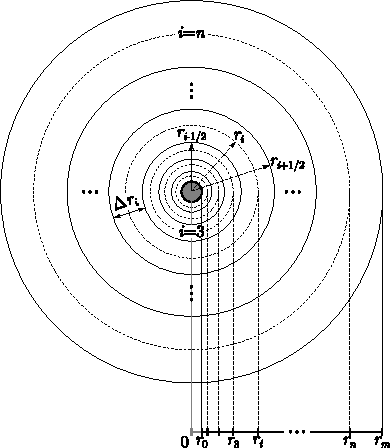
\includegraphics[width=9.5cm]{domain}
\caption{Schematic representation of the discretized domain considered in the model. $\Delta r$ is the variable segment size, increasing with the distance from the root surface ($r_0$) to the half-distance between roots ($r_m$), and $n$ is the number of segments}
\label{fig_scheme}
\end{figure}

\begin{figure}[h]
\centering
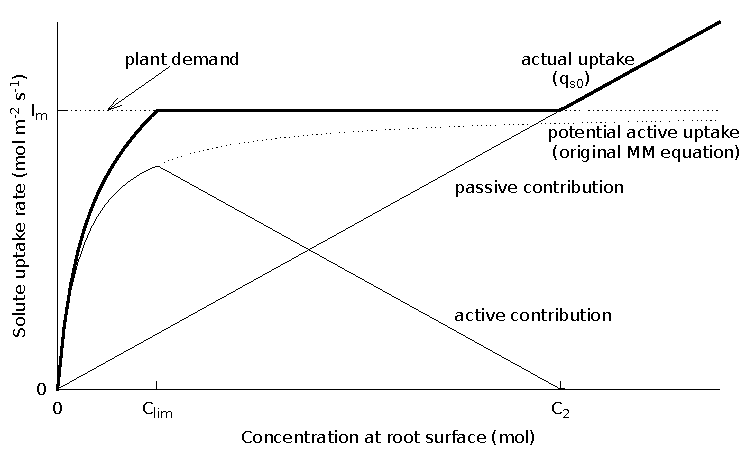
\includegraphics[width=13cm]{MM_c.pdf}
\caption{Solute uptake piecewise equation \ref{eq_MM_mod} from MM equation \ref{eq_MM1} with boundary conditions. The bold line represents the actual uptake, thin lines represent active and passive contributions to the actual uptake, and dotted lines represent the plant demand and the potential active uptake}
\label{fig_MM_mod}
\end{figure}




\end{document}
